\chapter{Stand van zaken}
\label{ch:stand-van-zaken}

% Tip: Begin elk hoofdstuk met een paragraaf inleiding die beschrijft hoe
% dit hoofdstuk past binnen het geheel van de bachelorproef. Geef in het
% bijzonder aan wat de link is met het vorige en volgende hoofdstuk.

% Pas na deze inleidende paragraaf komt de eerste sectiehoofding.


In dit hoofstuk zal er een stand van zaken gegeven worden van het onderwerp, hoe het vroeger gebeurde en hoe het tegenwoordig gebeurt. Eerst en vooral zal sectie \ref{sec:HCE} wat meer uitleg geven over HCE en hoe het simuleren van draadloze smart cards gebeurt. In sectie \ref{sec:NFC} zal een korte uitleg gegeven worden over NFC technologie. Ten slotte zal in sectie \ref{sec:Beveiliging} uitgelegd worden welke manieren er bestaan om HCE te beveiligen.


\section{Host-based Card Emulation (HCE)}
\label{sec:HCE}
Sinds de komst van Android 4.4 oftewel Android KitKat introduceerde Google een nieuwe technologie genaamd Host-based Card Emulation (HCE). HCE technologie maakt het mogelijk om Near Field Communication (NFC) technologie te gebruiken zonder de aanwezigheid van een secure element. 
Wanneer het Android toestel zich in card emulation (CE) mode bevindt en tegen een draadloze leer of point-of-sale (POS) terminal gehouden wordt, heeft het toestel de mogelijkheid om allerhande soorten draadloze smart cards te simuleren. Deze contactloze smart cards worden in vele situaties gebruikt zoals bij draadloos betalen, loyalty systemen, ticketing, toegang tot gebouwen,... ~\autocite{SCA2014}.

HCE maakt het dus mogelijk voor NFC apparaten om draadloze smart cards te simuleren. Om gebruik te kunnen maken van HCE heeft android verschillende libraries en APIs (Application Programming Interface) geimplementeerd in het besturingssysteem. Deze libraries en APIs worden overschreven door de applicaties die hier gebruik van willen maken en die op de CPU van het apparaat draaien, deze applicaties kunnen dan APDU (Application Protocol Data Unit) commando's en antwoorden uitwisselen met een NFC POS. Wanneer men vroeger gebruik wou maken van de NFC technologie kon dit alleen door een Secure Element (SE) die ingebouwd zat in het apparaat zoals een SIM kaart. De applicaties werden geïnstalleerd op dit SE die dan de APDU's afhandelde om zo draadloze smart cards veilig te kunnen simuleren. De APDU's die verstuurd worden van een NFC lezer worden opgevangen door de NFC antenne van het appparaat en wordt doorgegeven via de NFC controller naar het SE en omgekeerd zie figuur. Met HCE is het de bedoeling dat de nood van een SE verwijdert wordt uit deze operatie, ipv de APDU's door te geven naar het SE worden deze door gegeven naar de CPU van het apparaat en omgekeerd zie figuur ~\ref{fig:SE-HCE} ~\autocite{Alattar2014}. 

\begin{figure}
	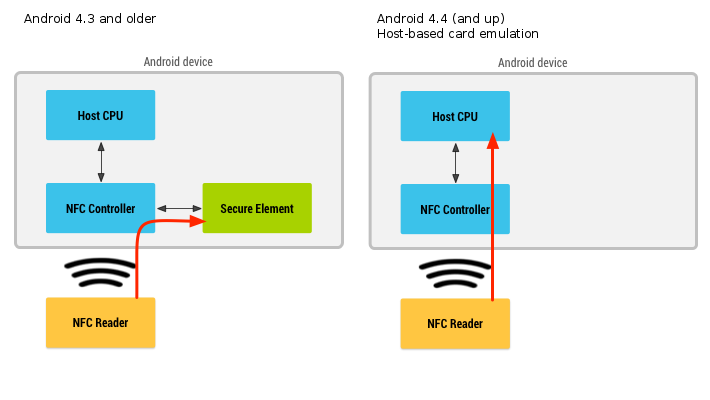
\includegraphics[width=\linewidth]
	{img/WalletHostBasedCardEmulation}
	\caption{Simulatie van een smart card via SE}
	\label{fig:SE-HCE}
\end{figure}


\section{Near Field Communication (NFC)}
\label{sec:NFC}
Near Field Communication (NFC) is een technologie die communicatie vanop korte afstanden, meestal nul tot vier centimeter maar kan tot 20 centimeter oplopen, mogelijk maakt. NFC apparaten kunnen actief of passief zijn, wanneer het NFC apparaat actief is dan gebruikt dit apparaat zijn eigen energiebron om zijn radio frequentie te genereren. Een passief NFC apparaat gebruikt de energiebron van een actief NFC apparaat om data te versturen, passieve NFC apparaten kunnen ook enkel maar antwoorden op aanvragen die vanaf een actief NFC apparaat verstuurd wordt. Transacties worden automatisch gestart door twee NFC apparaten elkaar te laten raken of deze twee dicht bij elkaar te houden ~\autocite{Alattar2014}. 

NFC heeft drie verschillende operating modes: Peer to Peer mode, Reader/Writer mode en Contactless Card Emulation. Peer To Peer mode biedt de mogelijkheid om data te versturen tussen twee NFC apparaten aan snelheden tot 424 Kbit/s. Reader/Writer mode maakt het mogelijk dat twee NFC apparaten gebruikt kunnen worden voor het lezen/schrijven van tags en draadloze smart cards, hierbij is de snelheid van het versturen van de data maar 106 Kbit/s. Contactless Card Emulation laat de NFC apparaten draadloze smart cards of tags simuleren die gelezen of naar geschreven kunnen worden door een NFC lezer ~\autocite{Alattar2014}. 

\section{Beveiliging HCE}
\label{sec:Beveiliging}
Met de komst van Host-base Card Emulation sinds Android 4.4 is er geen nood meer voor een Secure Element. HCE brengt wel een aantal beveiligingsrisico's met zich mee. Bij een simulatie van smart cards via SE wordt de applicatie geïnstalleerd op het Secure Element, aangezien het Secure Element hardware matig beveiligd is tegen fraude is de applicatie automatisch ook beveiligd tegen veiligheids bedreigingen. Wanneer er gekozen wordt voor een HCE gebaseerde simulatie wordt de applicatie gewoon op het apparaat geïnstalleerd en is deze niet meer beveiligd tegen bedreigingen van andere applicaties die ook op het apparaat staan.
Doordat de communicatie tussen de NFC controller en de HCE applicatie niet meer beveiligd is kan de communicatie tussen deze twee onderschept worden door andere malware applicaties. Malware applicaties vormen een groot gevaar voor uw Android toestel, deze malware applicaties kunnen het besturingssysteem aanval. Het risico van een aanval op het besturingssysteem wordt ook vergroot door exploiting, rooting of jailbreaking van het Android toestel. De malware applicatie kan ook de mogelijkheid hebben om exploiting, rooting of jailbreaking zelf te doen of de gebruiker in de val lokken om dit te doen ~\autocite{SCA2014}. 
Om deze bedreigingen tegen te gaan biedt de technologie de dag van vandaag een waaier van mogelijke oplossing die hiervoor ingezet kunnen worden:

\begin{itemize}
	\item White box cryptography
	\item Tamper proofed software
	\item Biometric factors
	\item Device identity solutions
	\item Security frameworks/trusted execution environment
	\item Encryption
	\item Tokenization
	\item Bijkomende beveiliging voorzien door een SE
\end{itemize}

\subsection{White Box Cryptography}
White box cryptography wordt gebruikt om geheimen/sleutels die in het geheugen of in code zitten te verbergen, het is een soort van verduistering die gebruikt wordt voor deterministische algoritmen, dit zijn algoritmen waarbij een bepaalde input altijd dezelfde output terug geeft, en wordt vooral toegepast op cryptografische algortimen. Bij white box implementaties wordt een cipher omgevromd tot een krachtige vorm waar het geheim/sleutel gecombineerd wordt met de code zodat het geheim/sleutel moeilijk afgeleid of herkent kan worden ~\autocite{SCA2014}.

\subsection{Tamper-Proofed Software}
Tamper proofing software is een extra beveiligingslaag in de software die ervoor zorgt dat het moeilijker is voor aanvaller om da code statische of dynamische aan te passen of reverse engineering te doen van de code. Dit kan gebeuren op verschillende manieren, runtime integrity checking, breakpoint defenses,  obfucation, anti-debug, ... Wanneer er een aanval wordt gedaan en ook effectief word waargenomen door de software zal het tamper-proofed systeem een antwoord produceren waardoor het programma niet goed meer werkt en de aanval wordt verhindert ~\autocite{SCA2014}.

\subsection{Biometric Factors}
Biometric factors of biometrische factoren kunnen gebruikt worden bij de authenticatie van een gebruiker in Host-based Card Emulation applicaties. Biometrische factoren worden meestal gebruikt in samenwerking met andere authenticatie middelen. Wat biometrische factoren zo aantrekkelijk maakt bij de authenticatie van gebruiker is voornamelijk de gebruiksvriendelijkheid, zeker in vergelijking met het bijhouden van meerdere wachtwoorden. Er bestaan verschillende soorten biometrische factoren die gebruikt kunnen worden: vingerafdruk, gezichtsherkenning, irisscan en stemherkenning. Deze biometrische factoren zitten al een tijdje geïntegreerd in de meeste laptops en smartphones en kunnen dus gemakkelijk op applicatie niveau gebruikt worden. Een bijkomend probleem is de privacy en beveiliging omtrent de biometrische data die ook in achting genomen zal moeten worden bij het implementeren van de applicatie ~\autocite{SCA2014}.

\subsection{Device Identity Solutions}
Device identity solutions gebruiken online diensten voor authenticatie van een toestel die zorgen voor een extra beveiligingslaag voor de Host-based Card Emulation applicaties. Fast Identity Online (FIDO) is een voorbeeld van zo een online dienst. FIDO maakt gebruik van publieke sleutel cryptografie technieken voor online authenticatie, het toestel van de gebruiken creëert een sleutel paar waarbij de privé sleutel bijgehouden wordt en de publieke sleutel geregistreerd wordt bij de online dienst. Het authentificeren van het toestel bij de online service wordt gedaan door middel van de privé sleutel die enkel lokaal ontgrendeld kan worden via biometrische factoren of door het ingeven van een PIN code.
FIDO ondersteunt veel verschillende technologieën die naaste elkaar gebruik kunnen worden zoals tokenisatie en one-time-password oplossingen. PayPal was een van de eerste die gebruik heeft gemaakt van vingerafdruk verificatie op de Samsung Galaxy S5 met FIDO Ready software ~\autocite{SCA2014}.

\subsection{Security Frameworks/Trusted Execution Environment}
\label{subsec:TEE}
Trusted Execution Environment (TEE) is een veilige plaats in de hoofd processor of coprocessor van het toestel waar data kan opgeslagen en verwerkt worden. De bedoeling van een TEE is het uitvoeren van geautoriseerde beveiligingssoftware in een vertrouwde omgeving. TEE bestaat niet enkel uit sofware maar ook uit hardware die bescherming bieden tegen aanvallen vanuit het rich operating system (Rich OS) in het toestel. Gevoelige applicatie die beschermt moeten worden van Rich OS worden opgeslagen in de TEE en helpt ook bij de controle van toegangsrechten tot de applicaties. TEE heeft zijn eigen besturingssysteem, hierdoor kan de TEE niet aangetast worden wanneer het besturingssysteem van het toestel aangetast is. De TEE kan voor een extra beveiligingslaag zorgen voor HCE applicaties ~\autocite{SCA2014}:

\begin{itemize}
	\item \textbf{PIN/wachtwoord ingave.} De TEE kan extra bescherming aanbieden aan de hand van het invoeren van een PIN code of een wachtwoord, bij de TEE is de invoer van de PIN code of een wachtwoord volledig gescheiden van de invoer van het toestel, hierdoor kan de invoer niet onderschept worden door malware applicaties die zich op het besturingssysteem van het toestel bevinden.
	
	\item \textbf{Secure storage of credentials.} De TEE implementeerd cryptografische operaties binnen de secure execution environment en zorgt voor het veilig opslaan van sleutels. Hierin kunnen dus tokens/sleutels van betalingsapplicaties in opgeslagen worden, zo zijn deze beter beveiligd tegen aanvallen dan wanneer ze opgeslagen worden in het besturingssysteem van het toestel.
	
	\item \textbf{Secure transfer protocol endpoint.} Het is mogelijk om in de TEE een geëncrypteerd beveiligd kanaal op te zetten van de kant van de terminal. Dit betekent dat de APDU's geëncrypteerd verstuurd kunnen worden van de terminal en de HCE applicatie via een draadloze interface naar de TEE. Een tweede geëncrypteerd beveiligd kanaal kan opgezet worden tussen de TEE en een Cloud applicatie. Hierdoor zijn de sleutels en data enkel zichtbaar binnen de vertrouwde applicatie, dit biedt een hoger niveau van beveiliging dan wanneer de applicatie uitgevoerd zou worden op het besturingssysteem van het toestel.
\end{itemize}

\subsection{Encryption}
Encryptie is een methode die het mogelijk maakt om data onleesbaar te versturen en niet als gewone tekst. Het ophalen van data die in gewone tekst verstuurd wordt is een van de grootste vormen van data breaches in card-present en card-not-present betalingsomgevingen, wanneer kaarten gelezen of de gegevens ingelezen worden in een web-based formulier. Er bestaan twee verschillende soorten encryptie end-to-end encryptie (E2EE) en point-to-point encryptie (P2PE), deze methodes zorgen ervoor dat de data geëncrypteerd is bij NFC lezer en het versturen van de data. Voor betalingsapplicaties can encryptie gecombineerd worden met tokenisatie (zie \ref{subsec:tok}), hierbij wordt het kaartnummer van een bankkaart geëncrypteerd en dan wordt het geëncrypteerde nummer gebruikt om een token te gaan genereren ~\autocite{SCA2014}.

\subsection{Tokenization}
\label{subsec:tok}
Tokenisatie is een methode die een willekeurige waarde teruggeeft van bijvoorbeeld een kaartnummer, rijksregisternummer, ... Tokenisatie op zich wordt al lang gebruikt maar heeft de laatste jaren meer aandacht gekregen door het toenemende aantal data breaches. Door het lekken van al die data is er een grote nood aan tokenisatie om betalingsgegevens te beschermen tegen fraude en vervalsing. Verschillende grote spelers binnen de beveiligingsindustrie hebben nieuwe standaarden opgesteld voor tokenisatie, één daarvan is EMVCo. De tokenisatie standaarden van die uitgebracht zijn door EMVCo voor betalingen kunnen heel domein specifiek zijn en bevat cryptogrammen die HCE use cases kunnen isoleren. Door dit toe te passen kan voorkomen worden dat de tokens gebruikt kunnen worden binnen andere betalingskanalen ~\autocite{SCA2014}.

\subsection{Secure Element}
HCE maakt het mogelijk om communicatie met de NFC controller te laten verlopen zonder een SE maar direct op de processor van het toestel, maar HCE specifieerd niet waar de data opgeslagen moet worden. De data kan zowel in de cloud als op een SE opgeslagen worden dus een combinatie van de twee is zeker ook mogelijk wanneer een SE aanwezig is in het toestel. Data die op het SE opgeslagen worden zijn beveiligd door het gebruik van cryptografische sleutels. De beveiliging van een SE kan nog versterkt worden door gebruik te maken van een TEE (zie \ref{subsec:TEE}). Het blijft wel nog altijd veiliger de applicatie en de data enkel op een SE uit te voeren en op te slaan ~\autocite{SCA2014}.


